\chapter{LHC and ATLAS}
\label{chap:cern}

The analyses presented in this thesis use the \gls{pp} collision data at a center-of-mass energy \cmtre TeV 
collected by the \gls{atlas} experiment in 2015, 2016 and 2017. 

The \gls{atlas} experiment is one of the four main experiments at the \gls{lhc} at the \gls{cern}. Section \ref{sed:cern:lhc} of this chapter describes the \gls{lhc} accelerator complex. This is followed by a general description of the detectors used in high-energy physics in Section \ref{sec:detectors}. The \gls{atlas} detector is discussed in Section \ref{sed:cern:atlas}.

%%%%%%%%%%%%%%%%%% LHC

\section{The Large Hadron Collider}
\label{sed:cern:lhc}

In this section we give a brief introduction to the \gls{lhc} \cite{1748-0221-3-08-S08001}, at the moment the largest and most powerful particle accelerator in the world, hosted by \gls{cern} and in operation since September 2008.
The first data for physics have been collected in the period  between 2010 and 2013, referred to as Run 1, at the center-of-mass energy of \cmsette and later 
\cmotto TeV, delivering to \gls{atlas} 5.5 \ifb at \cmsette TeV and 22.8 \ifb at \cmotto TeV.
After a shutdown of two years, in 2015 the \gls{lhc} started the Run 2 data taking at \cmtre TeV, which will continue until the end of 2018. 
In 2015--2017 the \gls{lhc} has delivered to \gls{atlas} 93 \ifb of \gls{pp} collisions. 

\subsection{A circular hadron collider}

The \gls{lhc} is a circular hadron accelerator, located in a 26.7 km long underground tunnel (with a depth ranging between 50 and 140 meters) that was previously hosting the \gls{lep}, a \gls{cern} accelerator that was operational from 1989 to 2000. The \gls{lhc} can accelerate protons up to a design center-of-mass energy of 13 TeV. Accelerating particles to very high energies is necessary both to study the structure of the particles themselves at smaller scales, and to create heavy states in collisions. Cosmic rays provide a source of particles with energies up to $10^7$ times higher than what the \gls{lhc} is capable of, but these extremely energetic rays are very rare, and is is not possible to modify the flux. 
Accelerators provide a well controlled flux of particles of a specific type in a specific location, and this allows the study of these particles with dedicated detectors.

A circular accelerator simplifies the acceleration of particles, as this can happen over several revolutions. When a charged particle travels on an orbit of radius $r$ under the effect of a magnetic field \textit{B}, its momentum $p$ is given by:
\begin{equation}
\label{eq:cern:p03br}
p = 0.3 r B,
\end{equation}
\noindent where the momentum is expressed in GeV, \textit{B} in Tesla and the radius of the orbit in meters. For a given magnetic field, a larger radius allows to reach higher energies. 

The choice of a collider over a fixed-target experiment is motivated by the possibility of reaching a higher energy in center-of-mass of the system: while in a fixed-target experiment this is proportional to the square root of the energy of the incoming particle, in a collider it is the sum of the energies of the two beams.


Suitable particles for a collider experiment need to fulfill two criteria: they need to be charged, in order to be accelerated and guided through electric and magnetic fields, and they need to be stable enough not to decay before being used for collisions. These criteria effectively limit the choice to protons, electrons, their antiparticles and ions. 

At the \gls{lhc} it has been chosen to study collisions with protons and lead ions. Three types of collisions are studied: \gls{pp}, lead-lead ($Pb$-$Pb$) and also proton-lead ($Pb$-$p$). The main reason to prefer protons over electrons is the energy loss that affects charged particles accelerated in a circular trajectory (syncrotron radiation), which decreases with the fourth power of the mass of the particle:

\begin{equation}
\label{eq:cern:sync}
\frac{dE}{dt} \propto \frac{E^4}{m^4 r^2} \; . \nonumber
\end{equation}

The larger mass of a proton with respect to an electron leads to a decrease by a factor $10^{12}$ in the energy lost through syncrotron radiation. This choice comes with a price: proton-proton collisions lead to less clean events, with a lot of soft interactions covering the interesting hard interactions. Furthermore, the center-of-mass energy is unknown as the particles taking part in hard interactions are not the protons themselves but their constituents.

\subsection{Magnet system} 


The \gls{lhc} is not a perfect circumference: it is composed of eight arcs (sectors), where the magnetic system is located, and eight straight sections containing the resonant cavities, the four interaction points with and the detectors, the equipment for beam injection and extraction, and other instrumentation. Magnetic fields are used to govern the trajectory of particles. In the \gls{lhc} there are more than nine thousand magnets, constructed from a superconducting alloy of niobium and titanium. About 150 tons of super-fluid helium at a temperature of 1.9 K are used to maintain the magnet system in the superconducting regime. Different types of magnets are necessary to achieve a proper control over the trajectory of particles.

\subsubsection*{Dipoles} 
Dipoles are used to create a vertical magnetic field, so as to bend the particles in the horizontal plane and thus give the dominant circular orbit. The \gls{lhc} has 1232 dipoles, each 15 m long and providing a magnetic field of 8.3 T. The current necessary to achieve this strong magnetic field is 11.8 kA.


\subsubsection*{Quadrupoles}
The \gls{lhc} has 858 quadrupoles, used for beam focusing. A single quadrupole can focus the beam either in the vertical or the horizontal plane, but it causes a defocusing in the other plane; conventionally a quadrupole is denoted as focusing if it is oriented to focus in the horizontal plane. A combination of focusing and defocusing quadrupoles separated by some drift space (FODO lattice) is used to keep both planes focused, and gives rise to Betatron oscillations. 

\subsubsection*{Higher-order magnets} 
Beside dipoles and quadrupoles, in the \gls{lhc} there are about 600 higher-order magnets that are used to maintain a good beam quality; e.g.  sextupoles are used to correct the spread in Betatron tune caused by the quadrupoles.



\subsection{Resonant cavities}

While the orbit of particles is governed by the magnetic fields, longitudinal electric fields are used for acceleration. In the \gls{lhc} the electric filed is provided by \gls{rf} cavities. There are overall 16 \gls{rf} cavities, eight per beam, hosted in four cryo-modules. Each cavity can provide an accelerating field of 5 MV/m, and oscillates with a frequency of 400 MHz. Since the electric field changes over time with the oscillations, particles passing through the same point of a \gls{rf} cavity at different times experience a different voltage; this produces a non-trivial longitudinal dynamics, where particles oscillate around the ideal synchronous particle with changes in momentum and phase (synchrotron oscillations). If we define the slip factor $\eta$ as the relative change in frequency in synchrotron oscillations with the relative change in momentum:
\begin{equation}
\eta = \frac{\Delta f / f}{\Delta p / p} \; , \nonumber
\end{equation}

\noindent and the compaction factor $\alpha$ as the relative change in frequency in orbit length with the relative change in momentum:

\begin{equation}
\alpha = \frac{\Delta L / L}{\Delta p / p} \; , \nonumber
\end{equation}

\noindent the following relation holds:

\begin{equation}
\eta = \frac{1}{\gamma^2} - \alpha \; , \nonumber
\end{equation}

\noindent where $\gamma$ is the Lorentz factor of the particle. This means that while the energy of the particle is low ($\eta>0$) an increase in momentum leads to an increase in frequency, while it leads to a decrease in frequency for $\eta<0$. At the transition energy, a previously stable synchrotron phase becomes unstable and vice versa; this requires a rapid change in \gls{rf} phase. This situation is illustrated in Figure \ref{fig:lhc:phase}(a). For example, a particle corresponding to the phase point A1 will arrive in the \gls{rf} cavity after one corresponding to the stability point P1, and will experiment higher voltage and increase in momentum; if $\eta>0$ this increase in momentum will translate in an increase in frequency and the particle will, at the following revolution, arrive earlier, while if $\eta<0$ the frequency will further decrease and the particle will be eventually lost.  The transition energy in the \gls{lhc} is 53 GeV, well below the injection energy of 450 GeV, so the \gls{lhc} is always above transition. 

\begin{figure}[ht]
\centering
\subfigure{\includegraphics[width=0.547\textwidth]{figures/Chap3/Rizzi-Fig3-1-1.pdf}}
\subfigure{\includegraphics[width=0.44\textwidth]{figures/Chap3/Rizzi-Fig3-1-2.pdf}}
\caption{(a) Phase stability below and above transition. (b) Bucket and the bunch for a beam above the transition energy. 
Figures based on the discussion in Ref. \cite{Tecker:2016mlq}.}
\label{fig:lhc:phase}
\end{figure}


In the \gls{lhc} beams particles are not distributed continuously, as this would not be allowed by phase instabilities, but are divided in bunches. 
The areas of stable motion are identified as bucket, and the area of the bucket is the beam longitudinal acceptance. 
The beam bunches fill only a part of the bucket, and the area of the beam bunches is the longitudinal beam emittance. Figure \ref{fig:lhc:phase}(b) shows a schematic view of the bucket and the bunch area for the case of a beam above the transition energy. 

\subsection{Luminosity and operational parameters}

The amount of data delivered by an accelerator is quantified by the integrated luminosity $\mathcal{L}_{int}$.
Given a certain process with production cross-section $\sigma$, the total number of events for that process is the product of cross-section and integrated luminosity:

\begin{equation}
\label{eq:cern:nev}
N_{\mathrm{events}} = \sigma \,\, \mathcal{L}_{int} \; . \nonumber
\end{equation}

The integrated luminosity is the time integral of the instantaneous luminosity $\mathcal{L}$, 

\begin{equation}
\label{eq:cern:intlumi}
\mathcal{L}_{int} = \int \mathcal{L} \, dt \; , \nonumber
\end{equation}

\noindent which, assuming a Gaussian particle distribution and the same characteristics for the two beams, can be expressed as:

\begin{equation}
\mathcal{L}=\frac{f N_b n^2}{4 \pi \sigma_{x}\sigma_{y} } \; , 
\label{eq:cern:lumi}
\end{equation}

\noindent where $f$ is the revolution frequency, $N_b$ the number of bunches in each beam, $n$ the number of protons in each bunch and $\sigma_{x(y)}$  is the transverse beam size at the interaction point in the $x$($y$) direction . 

The instantaneous luminosity defined in Equation \ref{eq:cern:lumi} needs to be corrected for two effects. First of all, this formula assumes a head-on collision between the bunches; in reality, to avoid unwanted interactions the beams collide with a crossing angle, and a large crossing angle decreases the instantaneous luminosity. The second correction is related to the beam transverse size, that can be expressed as:
\begin{equation}
\sigma_{x,y} = \sqrt{  \epsilon \beta^* } \; , \nonumber
\end{equation}
where $\epsilon$ is the beam emittance and $\beta^*$ is the beta function. Beam collisions happen in minibeta insertions, drift spaces with a beta waist in the center, where the beam size is as small as possible. In the vicinity of the minimum, the beta function evolves like:

\begin{equation}
\beta(s) = \beta^* + \frac{s^2}{\beta^*} \; . \nonumber
\end{equation}

From this it is possible to see that the smaller the beta function, the larger the dependence with $s$, so a bunch with a finite size will not have the same beta function as a whole (hour glass effect). This correction becomes more important with the decrease of the $\beta^*$ value. With the \gls{lhc} design parameters, the effect of crossing angle and hour glass changes the instantaneous luminosity by about 20\%.

The main limitations in the choice of the parameters that regulate the luminosity are collective effects, which could cause beam instabilities if the number of bunches or the number of protons per bunch is too high, and the limitations in the available aperture in the
quadrupoles focusing the beam in the minibeta insertions, that impacts $\beta^*$. The summary of the \gls{lhc} operational parameters during Run 2 is reported in Table \ref{tab:lhc:param}.


\begin{table}[ht]
\begin{center}
\begin{tabular}{c c c c c }
\hline 
Parameter & 2015 & 2016 & 2017 & Design \\ 
\hline 
\hline
Protons per bunch (n) [$10^{11}$ p] & $\approx$ 1.2 & $\approx$ 1.1 & $\approx$ 1.2 & 1.15 \\ 
\hline 
Number of bunches (N$_b$) & 2244 & 2220 & $\approx$ 2250 & 2780 \\ 
\hline 
Emittance ($\epsilon$) [mm mrad] & $\approx$ 3.5 & $\approx$ 2.2 & $\approx$ 2.2 & 3.5 \\ 
\hline 
Beta function ($\beta^*$) [cm] & 80 & 40 & 40 (30) & 55 \\
\hline
Crossing angle [$\mu$rad] & 290 & 370 (280) & 300 (340) & 285 \\
\hline
Peak luminosity [$10^{34}$ cm$^{-2}$s$^{-1}$] & 0.51 & 1.4 & 1.7(1.9) & 1.0 \\
\hline
\end{tabular}
\end{center}
\caption{\gls{lhc} operational parameters in Run 2 compared to their design value.
The numbers in parenthesis report changes in the parameters during the year. 
E.g. in 2016 the crossing angle was reduced after fill 5300,
while for 2017 the numbers in parenthesis report the values 
after the recommissioning with $\beta^* = 0.3$ m.}
\label{tab:lhc:param}
\end{table}


The luminosity profile changes over time, and different experiments have different luminosity needs. \gls{atlas} and CMS profit from having the maximum luminosity possible, while LHCb and ALICE have their top functionality at lower luminosity, and therefore apply a luminosity leveling that consists in changing the offset of the beams during the run, to maintain a constant (low) value of the instantaneous luminosity.

A high number of particles participating in a single bunch crossing can lead to a large number of multiple proton-proton collisions (pileup). In 2012 the \gls{lhc} operated with a bunch spacing of 50 ns, leading to a pileup of about 35 events per bunch crossing. With the increase in energy from Run 1 to Run 2, the same settings would have implied more than 100 events, above the limit for the proper functioning of the detectors. This is what motivated the choice to move from the 50 ns bunch spacing used in Run 1 to the 25 ns in Run 2: with this setup, for the same instantaneous luminosity is possible to have a lower ``per-bunch luminosity'' and therefore a lower pile up. Figure \ref{fig:atlas:pu} shows the luminosity-weighted distribution of the mean number of interactions per crossing during Run 1 (in Figure \ref{fig:atlas:pu:run1})
and in 2015--2017 (in Figure \ref{fig:atlas:pu:run2}) as recorded by the \gls{atlas} experiment.

\begin{figure}[ht]
\centering
\subfigure{\includegraphics[width=0.49\textwidth]{figures/Chap3/Rizzi-Fig3-2-1.pdf}\label{fig:atlas:pu:run1}}
\subfigure{\includegraphics[width=0.49\textwidth]{figures/Chap3/Rizzi-Fig3-2-2.pdf}\label{fig:atlas:pu:run2}}
\caption{Luminosity-weighted distribution of the mean number of interactions per crossing in 
\subref{fig:atlas:pu:run1} Run 1 and \subref{fig:atlas:pu:run2} Run 2 (2015--2017). All data recorded by \gls{atlas} during stable beams is shown. The mean number of interactions per crossing $\mu$ corresponds to the mean of the Poisson distribution of the number of interactions per crossing calculated for each bunch. It is calculated from the instantaneous per-bunch luminosity as 
$\mu = \mathcal{L}_{bunch}\sigma_{inel}/f$, where $\mathcal{L}_{bunch}$ is the per-bunch instantaneous luminosity, $\sigma_{inel}$ is the inelastic cross-section which is taken to be 80 mb for 13 TeV collisions, and $f$ is the \gls{lhc} revolution frequency. Figures from Ref. \cite{LumiTwiki}.}
\label{fig:atlas:pu}
\end{figure}


\subsection{Accelerator complex}

Protons are injected in the \gls{lhc} only after being accelerated to 450 GeV by a sequence of machines.

\begin{itemize}
\item Protons are extracted from $H_2$ at the Linac2 facility, a linear accelerator of 33 m that brings them to the energy of 50 MeV.
\item The \gls{psb} is the first synchrotron in the acceleration chain (with a circumference of 157 m), that in 1.2 s increases the energy of the protons from 50 MeV to 1.4 GeV.
\item With a circumference of 628 m, the \gls{ps} brings the protons to about 26 GeV. This was the oldest synchrotron experiment at \gls{cern}.
\item The \gls{sps} is the first accelerator of the chain to be underground (about 30 m) and has a circumference of 6.9 km; it brings the proton energy at 450 GeV. Beside preparing the protons to be injected into the \gls{lhc}, the \gls{sps} provides beam also to the North Area, 
where the beams for fixed-target experiments are prepared, 
and to the AWAKE experiment, that studies proton-induced plasma wakefield acceleration.
\item The \gls{lhc} is the last step of this chain, and it accelerates the protons form 450 GeV to 6.5 TeV (the design energy is 7 TeV); 
in the \gls{lhc} the protons gain about 0.5 MeV per turn, so it takes about 15 minutes to reach 6.5 TeV.
\end{itemize}

The accelerator complex of \gls{cern} is shown in Figure \ref{fig:lhc:acc}. The acceleration chain for lead ions differs from the one for protons in the initial part, which consists in Linac3  and \gls{leir} before the injection in the \gls{ps}. 

\begin{figure}[ht]
\centering
\includegraphics[width=1\textwidth]{figures/Chap3/Rizzi-Fig3-3.pdf}
\caption{ Schematic view of the \gls{cern} accelerator complex. The four main \gls{lhc} experiments are shown at the interaction points. Figure from Ref. \cite{Christiane:1260465}.}
\label{fig:lhc:acc}
\end{figure}

\subsection{Experiments at the LHC}

Seven experiments are built along the \gls{lhc} circumference and collect the data produced during the collisions. Each experiment is run by an independent collaboration that comprises several universities and research institutes. 
\gls{atlas} \cite{atlas:atlas} and CMS \cite{cms:cms} are the two largest and general purpose experiments, located at two opposite sides of the \gls{lhc} ring, in correspondence with two of the four interaction points. Their goal is to study a large variety of SM processes and to perform an extensive search program for \gls{bsm} physics. The independent design of the two detectors, as well as of the separation between the two collaborations running them, is essential to provide a validation of the \gls{lhc} results. Since the data used in this thesis is collected with the \gls{atlas} detector, a more extensive description of this experiment is given in Section \ref{sed:cern:atlas}. 
The LHCb \cite{lhcb:lhcb} and ALICE \cite{alice:alice} experiments are located at the other two \gls{lhc} interaction points. LHCb is a single-arm forward spectrometer, designed to perform high-precision studies of heavy flavor physics. The ALICE experiment is dedicated to the study of $Pb-Pb$ collisions, which at the \gls{lhc} happen with a center-of-mass energy of 2.6 TeV per nucleon pair; in this energy regime, quarks and gluons are expected to form a quark-gluon plasma.
The position of the four main experiments on the \gls{lhc} ring is shown in Figure \ref{fig:lhc:acc}.
Other three smaller experiments are installed along the \gls{lhc} circumference: TOTEM \cite{totem:totem}, LHCf \cite{lhcf:lhcf} and MoEDAL \cite{moedal:moedal}. TOTEM is located at the same interaction point as CMS, and measures the total \gls{pp} cross-section, as well as elastic and inelastic scattering. LHCf is installed in the same interaction point as \gls{atlas} and has two detectors, at 140 m from each side of the collision point, aiming at the study of particles produced in the ``forward'' region (very close to the beam axis). MoEDAL is installed in the LHCb cavern and is designed to search for magnetic monopoles.  


%%%%%%%%%%%%%%%%%% 

\section{Detectors for collider Physics}
\label{sec:detectors}

In this section we review the basic concepts that drive the design of the \gls{lhc} detectors, including \gls{atlas}.

\subsection{Identification of particles}
\label{sec:detectors:identification}



The ability to accurately identify particles and reconstruct their energy and trajectory is what drives the design of detectors for high energy physics. In a detector, different sub-systems are able to capture different types of particle interactions, and the combination of the information collected by each of them allows to identify particles (or at least assign them to families, such as neutral or charged hadrons). A typical schema of the subdetectors sequence is shown in Figure \ref{fig:detector:interaction}. The innermost layer, closer to the interaction point, is the tracking system, dedicated to the measurement of the signed charge and momentum of charged particles. The following layers are the electromagnetic and hadronic calorimeters, that measure the energy of particles with electromagnetic and hadronic interactions respectively. The outermost layer is dedicated to the muon system: because of their large mass (about 200 times more than electrons) muons do not produce electromagnetic showers and are therefore easy to identify as they are the only detectable particles that reach the external part of the detector.

\begin{figure}[ht]
\centering
\includegraphics[width=0.7\textwidth]{figures/Chap3/Rizzi-Fig3-4.pdf}
\caption{Components of a typical detector for physics at colliders. Different particles are identified by the distinctive signatures in the subdetectors.}
\label{fig:detector:interaction}
\end{figure}


\subsection{Tracking and spectrometry}
\label{sec:dec:tracking}
A tracking device measures the traces left by charged particles passing through it. To allow the determination of the momentum and the charge of a particle, a tracking device needs to be accompanied by a magnetic field (in this case we speak of a magnetic spectrometer): once the magnetic field is known, the measure of the radius of curvature of the particle is equivalent to a measure of its momentum, according to Equation \ref{eq:cern:p03br}. In a typical particle detector as the one in the schema in Figure \ref{fig:detector:interaction}, both the inner tracking system and the muon system are magnetic spectrometers.

The relative uncertainty in the momentum is given by:
\begin{equation}
\frac{\sigma_p}{p} = \sqrt{ \left(a p \right)^2 + b^2} \; .
\label{eq:tracking:reso}
\end{equation}

The first term, whose relative importance increases for high-momentum particles, derives from the resolution in the measurement of the curvature. Typical values for $a$ are between 0.01\% and 1\%. The constant term in Equation \ref{eq:tracking:reso} accounts for the impact of multiple Coulomb scattering, which broadens the distribution of the transverse momentum perpendicular to the direction of motion. This terms is important only at low energies, while it is negligible for high-energy particles.

There are three main configurations of magnetic fields typically used in momentum spectrometers:
\begin{itemize}
\item A dipole field leads to a rectangular symmetry; if we think of a circular collider with a coordinate system where $z$ is the direction along the beam trajectory and ($x$,$y$) define a Cartesian system in the transverse plane, a dipole  field in the $x$ direction will cause a deflection in the ($y,z$) plane. This is the configuration adopted by forward spectrometers like LHCb, where the tracking devices are arranged in sequence in the $z$ direction. As an example, the integral of the LHCb dipole field over the detector length is 4 Tm.

\item A solenoidal field leads to a cylindrical symmetry and, if the field lines are along the $z$ direction, the deflection is in the ($x,y$) plane. This is the typical configuration of the spectrometers in the central barrel, where the detectors are arranged in cylindrical layers. The CMS solenoid field is 4 T, while the \gls{atlas} one is 2 T. 

\item A toroidal field leads to an azymuthal symmetry: the direction of the field lines is a circle in the transverse plane, and the deflection is in the ($r,z$) plane. This configuration is adopted by the \gls{atlas} muon spectrometer, with a magnetic field of 4 T. As in the case of the solenoidal field, the detectors are arranged in cylindrical shells.
\end{itemize}

The track left by a charged particle curving because of the magnetic field is reconstructed by the tracking detectors. The two most common categories of tracking devices are gas and silicon detectors, described in the next two sections.

\subsubsection*{Gas detectors}

In gas detectors, the passage of a charged particle ionizes the atoms and creates electron-ion pairs. Once the electron and the ion are created, they can be separated (thus creating a current) by applying an electric field. This induces signal on an electrode added to the material, read through a readout system. The basic principle of most of gas detectors relies on a tube with a wire in the center, which is an anode with a high electric field. When the particle crosses the gas, the ionization electrons drift toward the anode and can be collected. 
Without an electric field, the electron and ion would move in the system by thermal diffusion. The effect of an electric field is to make the electron and ion move in opposite directions, allowing us to measure them. Since not many electrons are produced in gas, they need to be amplified. Inside the tube, the electric field decreases with the inverse of the distance from the anode wire. When the electrons reach a distance of a few micrometers from the wire, the electric field is very large and the electrons gain more energy than the ionization energy; this leads to secondary ionization and an exponential growth of the number of electron-ion pairs (avalanche effect). 

Several types of gas detectors with different characteristics have been developed. In single-wire proportional chambers, like the one used in the outer tracker of the LHCb experiment, several counters are combined next to each other, to allow the measurement of the particle position. In multi-wire proportional chambers \cite{CHARPAK1968262} several wires in two perpendicular directions are contained in the same box filled with gas. 
Drift chambers are a further evolution of wire chambers, where the position of the particle is computed by measuring the time taken by the 
secondary ionization to reach the anode. Time projection chambers (TPC) are a different type of gas detector, used for example in ALICE. 
It is constituted by a large area filled only with gas, without wires, with detectors and readout structure only at the end plates. 
Between the plates a strong electric field causes the electron-ion pairs to drift, 
until they reach the plates where a combined measurement of the position and time of arrival allows to reconstruct the three-dimensional 
trajectory of the particle (that can be curved if a magnetic field is added). 
Micro-strips chambers \cite{OED1988351} are more modern, very condensed and thin gas detectors. 
Instead of being generated by a wire, the electric field comes from small metal deposits on a high-resistivity substrate.   

In general the main problems of gas detectors based on ionization are the spatial extension and the long drift time, 
which nevertheless make them suitable for the outer part of the \gls{lhc} detectors, in particular muon spectrometers.

All the gas detectors described above are based on the electron-ion pairs created by the ionization induced by the charged particle. A different principle is used in \gls{trd}. \glspl{trd} are based on detecting the electromagnetic radiation emitted by particles that cross boundaries between different media below the Cherenkov threshold \cite{1402-4896-1982-T2A-024}. The energy radiated increases with the energy of the incoming particle. These detectors are less common for tracking, but are mentioned here as the main example of a modern \gls{trd} in high-energy physics is the \gls{trt} in the inner detector of the \gls{atlas} experiment.

\subsubsection*{Solid-state detectors}

Semiconductor (and in particular silicon) detectors are the main type of solid-state detectors, and are currently the most used for inner tracking, 
where high precision and low occupancy are needed \cite{Hartmann:2009zza}. 
These detectors detectors are also based on the ionization of the material but in this case, since the structure is a crystal, 
we talk about electrons and electron holes. 

The underlying principle is based on the band model of solids, describing the allowed energy levels for electrons in a solid: when many atoms of the same type are bound together in a crystal lattice, in order to fulfill Pauli's principle the atomic orbitals split into many closely spaced molecular orbitals, that can be considered as continuous energy bands. The highest-energy full band is the valence band, while the lowest partially-filled (or empty) band is the conduction band; the energy difference between the conduction band and the valence band is referred to as energy gap. 


Semiconductors are materials where the conduction band is almost empty, but the energy gap is small ($\approx$ 1 eV, e.g. 1.07 eV for silicon), so the conduction band can be occupied by excited electrons from the valence band; this leaves holes in the valence band, that under the effect of an electric field can drift as well. Semiconductors with a pure composition have the same amount of electrons and holes. If the semiconductor is doped with an atom with one more electron in the valence band, this creates an excess of electrons and the material is referred to as a n-type semiconductor. If instead the impurities are electron acceptors, the material has an excess of holes and is referred to as p-type semiconductor. When a p-type and a n-type semiconductors are pulled together, the holes of the p-side drift into the n-side, and the electrons from the n-side into the p-side. This creates an electric field that takes charge carriers out of the area where it is present (depletion region). When a charged particle passes through the semiconductor, it produces electron-hole pairs in the depletion region; these drift apart because of the electric field and can be collected by electrodes. The application of a negative potential difference between the p-side and the n-side can increase the depletion area.

The density of silicon is about one thousand times higher than that of gases like argon, and silicon also needs a much lower energy to be ionized (3.6 eV for silicon, while it is about 250 times higher for argon). This leads to a much higher number of electron-holes pairs than the number of electron-ion pairs in gas detectors, so the signal needs very little amplification, and the size of the detector itself can be smaller. 

Different configurations of the silicon sensors are possible. In a single-sided strip sensor, the readout strips are at negative potential. The second coordinate can be determined if also the n-side is divided into strips in a direction orthogonal to the ones in the p-side. 
The grid structure of this double-sided strip sensors can still lead to ambiguities when the number of hits is elevated; a true two-dimensional sensitivity is offered only by the pixel modules, where the module is divided in a matrix-like shape.



\subsection{Calorimetry}
\label{sec:dec:calo}

Calorimeters can determine the energy of both charged and neutral particles through a destructive measurement: the energy of the particles is deposited in the detector material and transformed into a measurable quantity. Because of their sensitivity to a wide variety of particles, good energy resolution and relatively small size, they are very attractive devices for accelerator physics experiments \cite{RevModPhys.75.1243,Wigmans:2000vf}.

When the incident particle interacts with the material of the calorimeter it develops a cascade of particles (shower), with different characteristics for electromagnetic and hadronic interactions, described in the next two sections. Different types of calorimeters are necessary to capture the two typologies. The energy of the shower is decreased by the interactions happening in the absorber material, while the active material provides the conversion of the energy into a charge or light signal. In sampling calorimeters layers of absorber and active material are alternated in sequence, while in homogeneous calorimeters a single material carries out both functions.


\subsubsection*{Electromagnetic calorimeters}

The type of interaction that electromagnetically interacting particles have with the detector depends on their energy. 
%As an example, the photon interaction cross-section in lead is shown in Figure  \ref{fig:det:xsec_photon}. 
%The average fractional energy loss in lead for electrons and positrons and the photon interaction cross-section in lead are shown in Figures \ref{fig:det:xsec_elec:a} and \ref{fig:det:xsec_elec:b} respectively. 

%\begin{figure}[ht]
%\centering
%\includegraphics[width=0.54\textwidth]{figures/Chap3/Rizzi-Fig3-5.pdf}
%\caption{Photon interaction cross-section in lead. Numbers from Ref. \cite{Nist}. }
%\label{fig:det:xsec_photon}
%\end{figure}

For photons and electrons with energies above 1 GeV, the dominant type of interaction is nuclear pair production and Bremsstrahlung, respectively. 
When these particles traverse a block of material they produce a cascade of particles (electromagnetic shower): electrons and positrons can emit a photon by Bremsstrahlung, and a photon, thanks to the interaction with a nucleus, can turn into an electron-positron pair.

The main parameter to describe the evolution of an electromagnetic shower is the radiation length ($X_0$), defined as the distance over which an electron reduces its energy to $1/e$ of the initial value, and it corresponds also to 7/9 of the mean free path for pair production for a photon. The radiation length depends on the characteristics of the material:
\begin{equation}
X_0 [\frac{g}{cm^2}] = \frac{716 \frac{g}{ cm^2} A }{Z(Z+1) \ln\left(287/\sqrt{Z}\right)} \; , \nonumber
\end{equation}

\noindent where $A$ and $Z$ are the atomic and mass number of the material. If we define $t = x/X_0$ as the shower depth relative to the radiation length, the maximum number of produced particles occurs at:
\begin{equation}
t_{max} = \frac{\ln\left(E_0/E_c\right)}{ln\left(2\right)} \;. \nonumber
\end{equation}
Typical values for the radiation length are of the order of the cm (e.g. 0.56 cm for lead, 1.76 cm for iron \cite{Patrignani:2016xqp}); 99\% of the shower is contained in about 11(22) $X_0$ for a particle with an energy of 1 GeV(TeV), 
allowing for electromagnetic calorimeters of compact dimensions. 
The lateral width of the shower, determined mainly by multiple scattering, increases with depth and is defined in terms of the Moli\`ere radius:
\begin{equation}
R_M = \frac{21 MeV \; X_0[\frac{g}{cm^2}]}{E_c [MeV]} \; . \nonumber
\end{equation}

\noindent A cylinder of radius 2$R_M$ contains about 95\% of the shower; for most calorimeters $R_M$ has a value of few centimeters, so electromagnetic showers are quite narrow. 

Once the electrons in the shower have an energy lower than the critical energy 
($E_c$, defined as the energy where the loss through Bremsstrahlung equals the loss through ionization), 
the shower stops as the energy is dissipated mostly through ionization for electrons and photoelectric effect for photons, 
and no longer through the creation of new particles. 
Therefore all the energy of the incoming particle is in the end used to ionize the material of the detector, and this is the effect that is detected.


We have discussed in Section \ref{sec:dec:tracking} how the resolution of the momentum measurement in a magnetic spectrometer decreases with the increase in the momentum itself. Instead, the relative energy resolution in a calorimeter improves for high-energy particles, and can be written in the parametric form:

\begin{equation}
\frac{\sigma_E}{E} = \sqrt{\left(\frac{a}{\sqrt{E}} \right)^2 + \left( \frac{b}{E} \right)^2 + c^2 } \; . \nonumber
\end{equation}

\noindent The first term of the sum in quadrature reflects the stochastic nature of the shower development: ignoring the instrumental effects, the energy resolution of a calorimeter is proportional to the square root of the total track length, which is in turn proportional to the initial energy. The contribution of this term is small in homogeneous calorimeters, while is larger in sampling calorimeters (because of fluctuations in the fraction of energy deposited in the absorber) and it grows with the thickness of the absorber layers; typical values for $a$ are 5-20\% if the energy is expressed in GeV. The second term is the noise term originating from the electronic noise of the readout chain; this term is in general more relevant for calorimeters producing charge signals than for those producing light signals, and can become the dominant term for particles with energy below 1 GeV. The last term is a constant deriving from instrumental effects that produce a non-uniform detector response, including for example energy lost outside the detector volume and radiation damage; this becomes the dominant term at high energies and is typically $<1\%$. 



\subsubsection*{Hadronic calorimeters}

The difference between electromagnetic calorimeters and hadronic calorimeters finds its origin in the more complicated nature of strong interactions compared to the electromagnetic ones. 

%A sketch of the evolution of a hadronic shower is shown in Figure \ref{fig:det:shower_had:a}. 
With respect to electromagnetic showers, hadronic ones have a much larger spatial extension. On the longitudinal direction, the scale is determined by the nuclear interaction length ($\lambda_I$), which is material-dependent and can be expressed as:
\begin{equation}
\lambda_I = 35 \frac{g}{cm^2} A^{1/3} \; , \nonumber
\end{equation}

\noindent where $A$ is the atomic number of the material. For most materials used in particle detectors this turns out to be larger than $X_0$ (e.g. the nuclear interaction length is 17.59 cm for lead, and 16.77 cm for iron \cite{Patrignani:2016xqp}). The 99\% shower containment is reached after about 5(9) $\lambda_I$ for pions with E=10(138) GeV. Also the lateral width of the shower is larger than in electromagnetic interactions: while the size of the Moli\'ere radius is determined mainly by multiple scattering, the lateral profile of a hadronic shower depends on the transverse-momentum transfer, which can be quite sizable in strong nuclear interactions. 
%Figure \ref{fig:det:shower_had:b} shows the lateral shower profile in iron for pions with E=10 GeV.

%\begin{figure}[ht]
%\centering
%\subfigure[]{\includegraphics[width=0.48\textwidth]{figures/Chap3/Rizzi-Fig3-6-1.pdf}\label{fig:det:shower_had:a}}
%\subfigure[]{\includegraphics[width=0.48\textwidth]{figures/Chap3/Rizzi-Fig3-6-2.pdf}\label{fig:det:shower_had:b}}
%\caption{\subref{fig:det:shower_had:a} Sketch of the evolution of a hadronic shower. Figure from Ref. \cite{grupen_shwartz_2008}. 
%\subref{fig:det:shower_had:b} Lateral energy distribution of shower induced by $\pi^-$ with E=10 GeV, measured at a depth of 10, 20, 30, 50 and 70 cm in Fe. Figure from Ref. \cite{FRIEND1976505}.}
%\label{fig:det:shower_had}
%\end{figure}


Another difference with electromagnetic showers lies in the composition of the shower: while an electromagnetic shower is constituted only by electrons, positrons and photons, a much larger variety of particles participates in hadronic showers, including both hadrons and electromagnetically-interacting particles. Starting from the simplifying assumption that one third of the particles produced in nuclear interactions are neutral pions ($f_{\pi^0}=1/3$), a first approximation of the electromagnetic fraction of a shower is given by:
\begin{equation}
f_{em} = 1 - \left(1 - \frac{1}{3} \right)^n \; , \nonumber
\end{equation}
where $n$ is the number of generations in the shower. Since the number of generations increases with the initial energy, it is intuitive that also $f_{em}$ will be larger for particles of higher energy. It is found \cite{GABRIEL1994336}:
\begin{equation}
f_{em} = 1 - \left(\frac{E}{E_0}\right)^{k-1} \; , \nonumber
\end{equation}
where $E_0$ is the energy necessary to produce one pion (e.g. 0.7 GeV for iron and 1.3 GeV for lead), and $k$ is a slope parameter related to $f_{\pi^0}$ through the average multiplicity ${<}m{>}$:
\begin{equation}
1-f_{\pi^0} = {<}m{>}^{k-1} \;. \nonumber
\end{equation}


%\begin{figure}[ht]
%\centering
%\subfigure{\includegraphics[width=0.42\textwidth]{figures/Chap3/Rizzi-Fig3-7-1.pdf}}
%\caption{Particle spectra produced by protons with E=100 GeV absorbed by lead, as simulated by the Fluka code \cite{Ferrari:898301} and averaged over many showers. Figure from Ref. \cite{RevModPhys.75.1243}.}
%\label{fig:det:shower_had_spectra}
%\end{figure}

%Figure \ref{fig:det:shower_had_spectra} shows 

If we consider e.g. the particle spectra produced by protons with E=100 GeV absorbed by lead, at low energies the particle content is dominated by electrons, positrons, photons and neutrons \cite{RevModPhys.75.1243}.

While in electromagnetic showers most of the initial energy is recorded in the detector, in hadronic showers a relevant fraction (up to 30-40\%) is invisible. This invisible fraction is caused by energy that goes into breaking the nuclear bonds, nuclear fragments that in sampling calorimeters do not reach the active material, and neutral particles that can escape the calorimeter (e.g. neutrinos or long-lived neutral kaons). Therefore, for the same initial energy, the visible energy will be lower for a hadronic shower than for an electromagnetic one. If we define the response as the collected signal per unit of incident energy, the invisible energy causes a different response of calorimeters to the electromagnetic and to the purely-hadronic parts of the shower. Defining $R_{em}$, $R_{h}$, $R_{\pi}$ respectively as the calorimeter response to electromagnetic shower, the hadronic part of the shower and to pions, we have that:
\begin{equation}
R_{\pi} = f_{em}R_{em} + (1-f_{em}) R_h = R_h \left( \frac{R_{em}}{R_{h}}f_{em} + (1-f_{em})  \right) \; . \nonumber
\end{equation}

In general, it is expected that $R_{em}/R_{h}>1$. Since the value of the electromagnetic fraction is energy-dependent, the signal from the calorimeter does not increase linearly with energy. Compensating calorimeters are aiming at having the same response to the electromagnetic and hadronic part of the shower ($R_{em}/R_{h}=1$), restoring the linearity of the calorimeter response. In non-compensating calorimeters the fluctuations in $f_{em}$ are the dominant component of the energy resolution and, since the fluctuations are approximately Gaussian,
they give rise to a term proportional to:

\begin{equation}
\frac{\sigma_E}{E} = \frac{\mathrm{const}}{\sqrt{E}}  \; . \nonumber
\end{equation}
In modern non-compensating calorimeters the value of the constant is about 0.4, while it can be as low as 0.2 in the case of compensating calorimeters.


\subsection{Detecting photons}

As already mentioned in previous sections, photons are often the result of the passage of a particle through the material; 
this is the case e.g. in \glspl{trd} or in calorimeters with scintillator as active material. 
This sections gives an overview of how these photons can generate a detectable current; for a more extensive discussion see e.g. Ref. \cite{lightdetection,Grupen:2012zpa}. The typical process of photon detection can be summarized in three different steps: (1) the incident photon generates a photoelectron or an electron-hole pair through the photoelectric or photoconductive effect, (2) the signal of the photoelectron is  
amplified, and (3) the amplified signal is collected. Important properties to classify photon-detecting devices are \cite{Patrignani:2016xqp}:
\begin{description}
\item[Quantum efficiency:] The probability that the incident photon generates a photoelectron. This depends on the photon wavelength.
\item[Collection efficiency:] The probability that the photoelectron is collected at the end of the chain.
\item[Photon detection efficiency:] The product of quantum and collection efficiency.
\item[Gain:] The amplification of the photoelectron, quantified as the number of electrons collected for each photoelectron generated.
\item[Dark current or dark noise:] The output current in the absence of signal.
\item[Energy resolution:] Resolution depending on electronic noise and statistical fluctuations.
\item[Dynamic range:] Maximum intensity that the detector can handle expressed in units of the smallest intensity with a signal-to-noise ratio above one.
\item[Time dependence:] Time between the arrival of the photon and the collection of the electrical current.
\item[Rate capability:] Inverse of the time needed after the arrival of a photon to be ready for another one.
\end{description}

Photon detectors can be broadly classified into three categories: vacuum, gaseous and solid-state detectors, described in the following paragraphs.

\subsubsection*{Photomultiplier tubes}  

\Glspl{pmt} are the most common type of vacuum photon detectors. 
A sketch of the structure of a \gls{pmt} is shown in Figure \ref{fig:det:pmt}. It consists of a vacuum tube with an input window, a photocatode, 
a focusing electrode, electron multipliers, and an anode  \cite{hamamatsu}. 
Photons enter the device through the window and excite the electrons in the valence band of the photocatode, which is a semiconductor; 
in transmission-type \glspl{pmt} the photocatode is deposited on the inside of the window, 
while in reflection-type \glspl{pmt} it is on a separate surface. 
The excited electrons diffuse to the surface of the semiconductor and, if they have enough energy to overcome the vacuum level barrier, 
are emitted as photoelectrons. These are accelerated and focused by the electrode toward the multi-stage dynodes, 
a system of electrodes coated with a secondary emissive material, 
where the incident electrons are multiplied. 
The gain $G$ of the \gls{pmt} depends on the applied voltage $V$ as $G=AV^{kn}$, 
where $A$ and $k$ are constants and $n$ is the number of multiplicative stages. 
Typical values for the gain are $10^5-10^6$. After the last stage of multiplication, the electrons are collected by the anode, 
which then outputs the current to the external circuit.

\begin{figure}[ht]
\centering
\subfigure{\includegraphics[width=0.8\textwidth]{figures/Chap3/Rizzi-Fig3-8-1.pdf}}
\caption{Sketch of the structure of a \gls{pmt}. }
\label{fig:det:pmt}
\end{figure}

Beside \glspl{pmt}, other examples of vacuum photon detectors are \gls{mcp} and \gls{hpd}. \glspl{mcp} are based on the same principle as \glspl{pmt} but substitute the discrete multiplicative stages of the dynodes with continuous multiplication in cylindrical holes of a few $\mu$m. The decreased size of a \gls{mcp} comes at the price of a large recovery time, shorter lifetime and smaller gain (typically $\approx 10^4$). In \glspl{hpd} photoelectrons are accelerated onto a silicon sensor, allowing higher resolution in space and energy; this type of sensors are used e.g. in the \gls{cms} hadronic calorimeter.

\subsubsection*{Gaseous photon detectors}
In gaseous photon detectors the photoelectrons are multiplied through the avalanche effect in an high-field region, similarly to what happens in gaseous tracking detectors. The photoelectrons are generated by the interaction of the photon either with a solid photocatode or with a photosensitive molecule vaporized and mixed in the gas itself. 

\subsubsection*{Solid-State photon detectors}
Solid state photon detectors are devices where the production and detection of the photoelectrons takes place in the same semiconductor material. They are in rapid development (see e.g. Ref. \cite{Renker:2009zz}) as they provide a smaller, and often cheaper, option to \glspl{pmt} and gaseous detectors, especially when the area to be covered is small. 
Silicon photodiodes are devices based on a reverse-biased p-n junction, used in many applications from high-energy physics to solar cells. 
Photons passing through the silicon create electron-hole pairs through the photoconductive effect, which are then collected respectively at the positive and negative side of the chip. 

 %Advances in solid state photon detectors




%%%%%%%%%%%%%%%%%% ATLAS

\section{The ATLAS experiment}
\label{sed:cern:atlas}

\gls{atlas} \cite{atlas:atlas}, shown in Figure \ref{fig:atlas:atlas}, is the largest of the \gls{lhc} detectors, 
measuring 44 meters in length and 25 meters in height, and weighting about 7000 tons. 
To be fully functional in the \gls{lhc} environment,  the \gls{atlas} detector needs to be fast in order to resolve the collisions resulting from consecutive bunches (which are interspaced by 25 ns) and radiation resistant. 

\begin{figure}[ht]
\centering
\subfigure{\includegraphics[width=0.85\textwidth]{figures/Chap3/Rizzi-Fig3-9-1.pdf}}
\caption{Drawing of the \gls{atlas} detector showing the different subdetectors and
the magnet systems. Figure from Ref. \cite{atlas:atlas}.}
\label{fig:atlas:atlas}
\end{figure}

The \gls{atlas} physics program covers a large variety of topics: 
\begin{itemize}
\item \gls{sm} processes can be measured at the \gls{lhc} at energies never reached before, and being sensitive to them is essential both to provide accurate measurements and to use them as candles to calibrate the detector. 
\item The discovery of the Higgs boson was one of the main goals of the \gls{lhc} and, after its observation in 2012, the focus moved onto measuring its properties. 
\item Compared to the Tevatron, the \gls{lhc} is a true top-quark factory, 
and the study of the properties of this particle can both probe the \gls{sm} and set limits on \gls{bsm} theories.
\item The \gls{lhc} offers an exciting opportunity to discover \gls{bsm} physics, and \gls{atlas} needs to be ready to identify its signs. 
\item \gls{atlas} has a dedicated program to study the properties of the physics involving \textit{b}- and \textit{c}-quarks, and of the physics of low mass states.  
\item \gls{atlas} also carries out a heavy-ion program.
\end{itemize}

To cope with the wide range of types and energies (from few GeV to several TeV) of particles that need to be identified, \gls{atlas} relies on a sequence of subdetectors nested in a cylindrical geometry, that follow the general schema discussed in Section \ref{sec:detectors:identification}: close to the \gls{ip} we find the \gls{id}, embedded in a solenoidal magnetic field of 2 T. The following layers are the \gls{ecal} and \gls{hcal}, and the outermost part is occupied by the muon system, where muons are bent by a 4 T toroidal magnetic field. All these components are described in the next sections.

\subsection{Coordinate system}

\gls{atlas} uses a right-handed coordinate system, with its origin at the nominal \gls{ip}. The $z$-axis follows the beam direction, 
while in the transverse plane the $y$-axis points upward and the $x$-axis toward the \gls{lhc} center. Positive and negative values of the $z$-axis identify respectively the A-side and the C-side of the detector. 
When spherical coordinates are used, the azimuthal angle $\phi$ is defined starting from the $x$-axis, 
and ranges between $-\pi$ and $\pi$; the polar angle $\theta$ is defined starting from the $z$-axis and takes values between $0$ and $\pi$. 
The pseudorapidity is often used instead of the polar angle and is defined as: 
 
\begin{equation}
\eta = - \ln\tan\left(\frac{\theta}{2}\right) \; . \nonumber
\label{eq:cern:eta}
\end{equation}

\noindent In the limit of massless particles, is equivalent to the rapidity:

\begin{equation}
y = \frac{1}{2} \ln\left(\frac{E + p_z}{E - p_z}\right) \; , \nonumber
\label{eq:cern:y}
\end{equation}

\noindent where $E$ is the energy of the particle and $p_z$ its momentum projected on the $z$-axis. 
The advantage of rapidity and pseudorapidity over the polar angle is that rapidity differences $\Delta y$ are boost-invariant 
along the $z$-axis, as well as pseudorapidity differences $\Delta \eta$ for massless particles.
The pseudorapidity is usually preferred to the rapidity as it does not require
knowing the particle’s mass but only its polar position.
The $\eta$-$\phi$ plane is used to define the angular separation of two objects in the detector:

\begin{equation}
\Delta R = \sqrt{ (\Delta \eta)^2 + (\Delta \phi)^2  } \; . 
\label{eq:cern:dR}
\end{equation}

Since protons are composite particles, and the hard scattering happens between its constituents, the longitudinal momentum of the partons is unknown. It is therefore useful to define the transverse momentum (\pt) as the projection of the momentum on the ($x$,$y$) plane: 

\begin{equation}
\pt = \sqrt{p_x^2 + p_y^2} \; , \nonumber
\label{eq:cern:pt}
\end{equation}

\noindent where $p_{x(y)}$ are the projection of the momentum along the $x$-($y$-)axis.



\subsection{Magnet system}
\label{sec:atlas:magnets}

The two segments of the \gls{atlas} detector that are dedicated to tracking, the \gls{id} and the muon spectrometers, are embedded in two separate magnetic fields. A schematic overview of the \gls{atlas} magnetic system is shown in Figure \ref{fig:atlas:magnet}.
\label{sec:cern:atlasmagnets}
\begin{figure}[ht]
\centering
\subfigure{\includegraphics[width=0.85\textwidth]{figures/Chap3/Rizzi-Fig3-10-1.pdf}}
\caption{Layout of the \gls{atlas} magnet system. Figure adapted from Ref. \cite{Goodson}.}
\label{fig:atlas:magnet}
\end{figure}

As discussed in Section \ref{sec:dec:tracking}, the magnetic field configurations that are more suitable for a detector with cylindrical symmetry are solenoidal and toroidal. The bending of the charged particles in the \gls{atlas} \gls{id} is caused by an axial 2 T solenoidal field, provided by the central solenoid \cite{YAMAMOTO200853}. This magnet is 5.8 m long, has an inner diameter of 2.46 m and an outer diameter of 2.56. The wounded coil is made of an Al-stabilized NbTi conductor, and is powered with a 7.73 kA current. 


In the muon system, a solenoid would be disadvantageous in the measurement of forward muons, since the resultant magnetic field would not be perpendicular to the trajectory of those particles. The usage of a toroid to provide the outer magnetic field solves this problem. 
The choice of the “open air” toroid configuration allows a good muon
reconstruction performance without relying on the \gls{id}. 
The toroids allow to efficiently generate the magnetic field over a large volume with a reduced amount
of material. This minimizes the amount of multiple scattering, which represents one
of the factors limiting the muon momentum resolution.
The main drawback of the usage of a toroid is that, in order to obtain the same strength of magnetic field, a toroid needs more current than a solenoid (20.5 kA for 4 T).
The \gls{atlas} toroid system is divided into two subsystems, to allow for an easier design, 
as well as to provide access to the core part of the detector.
The barrel toroid \cite{ATLAS:1997ac} provides a peak field of 3.9 T in the cylindrical shell between the calorimeters and the end of the muon spectrometer, and consists of eight coils contained in individual vacuum vessels.  
The end-cap toroids \cite{ATLAS:1997ab} provide the magnetic field necessary to bend the muons in the end-cap region of the spectrometer, and each of them consists of eight coils building a single cold mass, originating a peak field of 4.1 T. 



\subsection{Inner detector}
\label{sec:atlas:id}

The main purposes of the \gls{atlas} \gls{id} \cite{ATLAS:1997ag,ATLAS:1997af} are to provide a good momentum resolution of the charged particles produced in the collisions and to allow the determination of secondary vertices. The dimensions of the \gls{id} are determined on one side by the 
radius of the beam pipe and on the other side by the beginning of the \gls{ecal}. The total length is 5.4 m, which provides a coverage up to $|\eta|<$2.5.
The \gls{id} is divided into a barrel, whose schema is shown in Figure \ref{fig:atlas:id}, and two end-cap regions, covering respectively the pseudorapidity regions $|\eta|<1.2$ and $1.2<|\eta|<2.5$. In both, a mixture of gaseous and silicon detectors is used to maximize the performance and reduce the costs. The three components of the \gls{id} are the pixel detector, the semi-conductor tracker, and the transition radiation tracker, discussed in the following paragraphs.

\begin{figure}[ht]
\centering
\subfigure{\includegraphics[width=0.65\textwidth]{figures/Chap3/Rizzi-Fig3-11-1.pdf}}
\caption{Layout of the \gls{atlas} \gls{id}. Figure from Ref. \cite{Potamianos:2016ptf}.}
\label{fig:atlas:id}
\end{figure}


\subsubsection*{Pixel detector}
\label{sec:atlas:pixel}
The innermost layer of the \gls{id} is the pixel detector \cite{Aad:2008zz}, divided into barrel and end-cap regions. 
During the Long Shutdown after the \gls{lhc} Run 1, the \gls{id} was subject to important upgrades \cite{Potamianos:2016ptf}. 
The main one is the addition of a fourth pixel layer in the barrel, in addition to the three already existing ones, 
the \gls{ibl} \cite{Capeans:1291633}, that is positioned 3.33 cm away from the \gls{ip}. 
In order to locate a detector so close to the \gls{ip}, the beam pipe had to be replaced with a thinner one. 
The \gls{ibl} is 72.4 cm long along the $z$-direction, and consists of 14 staves that provide full coverage in azimuthal angle. Each stave contains 20 modules, 12 with planar silicon sensors and eight with 3D pixel sensors \cite{1748-0221-7-11-P11010}, and each module has 144$\times$328 pixels with an area of 50$\times$250 $\mu$m$^2$ and a depth of 200 $\mu$m and 230 $\mu$m for the planar and 3D sensors respectively, 
for a total of over 12 million pixels in the entire \gls{ibl}. The size of the pixels leads to a resolution of 40 and 8 $\mu$m respectively in the longitudinal and transverse direction. 
The three outer pixel layers are located at 5.05, 8.85 and 12.5 cm from the \gls{ip}. 
Each module contains 80 pixels with an area of 50$\times$400 $\mu$m$^2$ and a depth of 250 $\mu$m, leading to a spatial resolution of 115 and 10 $\mu$m respectively in the longitudinal and transverse direction. 
The two end caps, on the two sides of the detector, consist of three wheels each, with a radius of 34 cm and located at 49.5, 58.8 and 65.0 cm from the \gls{ip}. 
To ensure a good performance, the pixel detectors need to be kept at a low and stable temperature, 
between -15$^{\circ}$ C and 5$^{\circ}$ C for the \gls{ibl}, and between -15$^{\circ}$ C and -10$^{\circ}$ C for the other layers.

\subsubsection*{Semi-conductor tracker}
The \gls{atlas} \gls{sct} is composed by 4088 silicon micro-strip modules with binary readout mounted on carbon fibre composite structures, and is organized in four cylinders in the barrel and nine disks in each of the forward regions \cite{Jackson:sct}. The cylinders have  radii of 30.0, 37.3, 44.7 and 52.0 cm and provide a coverage for $|\eta|<1.1-1.4$, while the disks cover the region with $1.1-1.4<|\eta|<2.5$. 
Out of the 4088 \gls{sct} modules, 2112 modules are in the barrel, 
and contain single-sided p-in-n silicon strips, with a pitch of 80 $\mu$m. 
In each module, the strip sensors are positioned back to back with an angle of 40 mrad, to be able to access information on the $z$-coordinate as well. The end-cap modules use strips with width between 56.9 and 94.2 $\mu$m. 
These choices lead to a spatial resolution of 580 $\mu$m in the longitudinal direction and 17 $\mu$m in the transverse one.
Also the \gls{sct} components need to be kept at a low temperature, between -15$^{\circ}$ C and -5$^{\circ}$ C.

\subsubsection*{Transition radiation tracker}

The \gls{trt} is the outermost layer of the \gls{id}. In the barrel it consists of 52544 straw tubes with a length of 1.5 m disposed parallel to the beam direction, while each end-cap contains 122880 straw tubes 0.4 m long disposed perpendicularly to the beam axis. Each tube is 4 mm in diameter, and has in the inside gold plated tungsten wire as anode with a diameter of 31 $\mu$m. The tubes are filled with a mixture of 70\% Xe, 27\% CO$_2$ and 3\% O$_2$; due to a gas leakage, in 2016 part of the \gls{trt} tubes have been filled with a cheaper mixture of 80\% Ar and 20\% CO$_2$. The \gls{trt} has a pseudorapidity coverage up to $|\eta|<2$ and it provides tracking information only in the (r-$\phi$) plane, with a resolution of 130 $\mu$m.


\subsection{Calorimeters}
\label{sec:atlas:calo}

The \gls{atlas} calorimeter system is located outside the \gls{id} and the magnetic field of the solenoid, as shown in Figure \ref{fig:atlas:calo}. The \gls{ecal} is closer to the \gls{ip}, while the \gls{hcal} is on the outside; both systems have a barrel and an end-cap section. 
The combined thickness of the calorimeter system is about 11 interaction lengths to ensure the longitudinal containment of energetic jets, 
as well as a good reconstruction of the energy imbalance in the event, which is a measure of the energy carried away by neutral weakly-interacting particles. The total pseudorapidity coverage is up to $|\eta|<4.9$. 

\begin{figure}[ht]
\centering
\subfigure{\includegraphics[width=0.75\textwidth]{figures/Chap3/Rizzi-Fig3-12-1.pdf}}
\caption{Layout of the \gls{atlas} calorimeter system. Figure from Ref. \cite{atlas:atlas}.}
\label{fig:atlas:calo}
\end{figure}

Table \ref{tab:atlas:cal:reso} summarizes the energy resolution of the different subsystems. As expected from the discussion in Section \ref{sec:dec:calo}, the resolution is better for electromagnetic showers than for the hadronic ones. For example, a 1 GeV particle detected in the \gls{ecal} has an energy resolution of about 19\%, while 50\% (100\%) if detected in the \gls{hcal} barrel (end-caps). On the other hand, a 1 TeV particle has an energy resolution of 0.7\% in the \gls{ecal} and 3\% (10\%) in  \gls{hcal} barrel (end-caps), and in this case the resolution is dominated by the constant term, 
related to instrumental effects and to the different response of the detectors to electromagnetic and hadronic showers. 

\begin{table}[ht]
\begin{center}
\begin{tabular}{c c }
\hline
Component & $\sigma_E / E$ \\
\hline 
\hline
\gls{ecal} & 0.1$/\sqrt{E[GeV]}$ $\bigoplus$ 0.17$/E$ $\bigoplus$ 0.007 \\ % chiara: cite LAr TDR
\hline
\gls{hcal} barrel & 0.5$/\sqrt{E[GeV]}$ $\bigoplus$ 0.03 \\
\hline
\gls{hcal} end caps & 1$/\sqrt{E[GeV]}$ $\bigoplus$ 0.1 \\
\hline
\end{tabular}
\end{center}
\caption{Energy resolution of the \gls{atlas} calorimeters.}
\label{tab:atlas:cal:reso}
\end{table}

\begin{figure}[ht]
\centering
\subfigure[]{\includegraphics[width=0.495\textwidth]{figures/Chap3/Rizzi-Fig3-13-1.pdf}}
\subfigure[]{\includegraphics[width=0.495\textwidth]{figures/Chap3/Rizzi-Fig3-13-2.pdf}}
\caption{(a) Schema of a barrel module of the \gls{atlas} \gls{ecal}. Figure from Ref. \cite{atlas:atlas}. (b) Accordion shape of the metal plates of the \gls{ecal}.}
\label{fig:atlas:lar}
\end{figure}

\subsubsection*{Electromagnetic calorimeter}

The \gls{ecal} is a sampling calorimeter with \gls{lar} as active material and lead plates as absorber, both in the barrel and in the end caps. The lead plates have a characteristic accordion shape and, in the barrel, are oriented in the radial direction. Before the \gls{ecal}, a presampler provides the information necessary to reconstruct the amount of energy lost in the passive material of the solenoid. The design of a \gls{lar} barrel module is shown in Figure \ref{fig:atlas:lar}(a), where it is possible to see the segmentation in three layers with decreasing granularity: the first layer is finely segmented in pseudorapidity, with strips of $\Delta\eta \times \Delta\phi = 0.0031 \times 0.098$; the second layer has towers of $\Delta\eta \times \Delta\phi =  0.025 \times 0.025$ to measure the clusters, while the third layer has wider towers of $\Delta\eta \times \Delta\phi =  0.05 \times 0.0245$ to provide an estimate of the energy leaking outside the \gls{ecal}. The \gls{lar} barrel offers pseudorapidity coverage up to $|\eta|<$1.475, and the thickness of the detector varies from 22 $X_0$ at $\eta=0$ to 33 $X_0$ at $|\eta|=1.3$. 
Each of the two end-cap regions consists of two coaxial wheels, of eight modules each, that cover the region $1.375<|\eta|<3.2$, with a thickness varying between 26 and 36 $X_0$ for the inner wheel and between 24 and 38 $X_0$ for the outer wheel. The end-cap modules are divided into two layers, again with decreasing granularity.


\subsubsection*{Hadronic calorimeter}

The hadronic calorimeter is composed of three subsystems with different technologies: the \gls{tilecal} \cite{TileTDR} is a sampling calorimeter with plastic scintillator as active material and steel as absorber, the hadronic end-cap calorimeter (HEC) uses copper as absorber and liquid argon as scintillator, while the forward calorimeter (FCal) also uses liquid argon in the active layer but has tungsten rods embedded in a copper matrix as absorber. The choice of the materials is driven by the need to have detectors more resistant to radiation in the forward region, where the flux of particles is larger. 

\gls{tilecal} covers the pseudorapidity region with $|\eta|<1.7$, and is divided into a central \gls{lb}, 5.8 m long, and two \glspl{eb}, 2.6 m long; the \gls{tilecal} inner radius is 2.28 m, and the outer radius 4.25 m. Each barrel is divided in 64 modules, disposed on the $\phi$ direction and each having the size of 0.1 radians. Each module is further segmented radially into three layers with thicknesses of about 1.5, 4.1 and 1.8 $\lambda_I$ in the \gls{lb} and 1.5, 2.6 and 3.3 $\lambda_I$ in the \gls{eb}; a schematic of one module is shown in Figure \ref{fig:atlas:tile}(a). Ionizing particles passing through the plastic scintillator (polystyrene) produce ultra-violet light, which is then collected at the two edges of each tile and converted to the longer wavelength of visible light by wavelength-shifting fibers. The fibers, with a diameter of 1 mm each, transmit the light to the readout \glspl{pmt} located in the grinder.

\begin{figure}[ht]
\centering
\subfigure[]{\includegraphics[width=0.4\textwidth]{figures/Chap3/Rizzi-Fig3-14-1.pdf}}
\subfigure[]{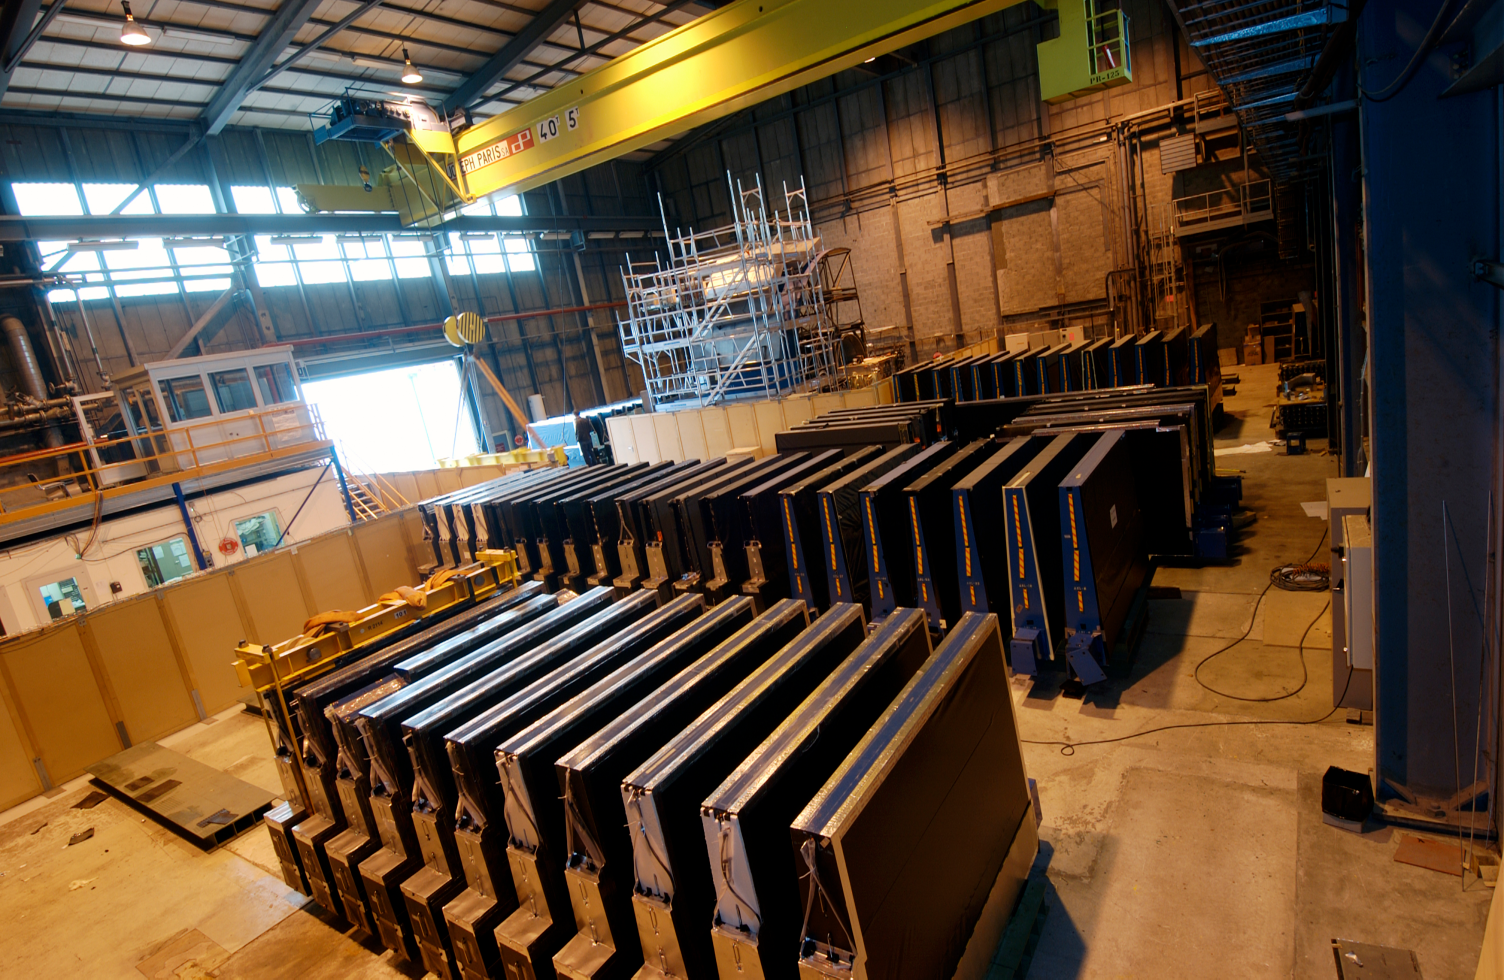
\includegraphics[width=0.59\textwidth]{figures/Chap3/Rizzi-Fig3-14-2.pdf}}
\caption{(a) Schematic representation of a \gls{tilecal} module and its interface with the optical readout. Figure from Ref. \cite{atlas:atlas}. (b) \gls{tilecal} modules before the installation.}
\label{fig:atlas:tile}
\end{figure}

An approximately projective geometry, shown in Figure \ref{fig:atlas:tile_cells}, is provided by the grouping of the readout fibers into the \glspl{pmt}: this defines a cell structure, and each cell has dimension $\Delta\eta \times \Delta\phi = $ 0.1 $\times$ 0.1 in the first two layers and $\Delta\eta \times \Delta\phi = $ 0.2 $\times$ 0.1 in the third layer. Special cells cover the gap region between the \gls{lb} and the \gls{eb}: the gap scintillators in the pseudorapidity region $1.0<|\eta|<1.2$ and the crack scintillators in the region $1.2<|\eta|<1.6$, in front of the \gls{lar} end caps.

\begin{figure}[ht]
\centering
\subfigure{\includegraphics[width=1.0\textwidth]{figures/Chap3/Rizzi-Fig3-15-1.pdf}}
\caption{Layout of the projective geometry of the \gls{tilecal} cells. Figure from Ref. \cite{atlas:atlas}.}
\label{fig:atlas:tile_cells}
\end{figure}

The HEC shares the same cryogenic system as the \gls{ecal} end caps, and covers the region with $1.5<|\eta|<3.2$. Liquid argon is more resistant to radiation than the plastic scintillator used in \gls{tilecal}, and is therefore the preferred choice in the end-cap region. Each side of the HEC consists of two wheels with outer radius of 2.03 m, and each wheel is composed by 32 identical modules. The electromagnetic signal produced in the \gls{lar} is collected by cathodes on the plates. 

The FCal provides coverage in the forward region with $3.1<|\eta|<4.9$. The FCal modules are located at high pseudorapidity, at a distance of 4.7 m along the $z$-axis from the \gls{ip}.


\subsection{Muon spectrometer}

The \gls{ms} \cite{ATLAS:1997ad}, shown in Figure \ref{fig:atlas:muon}, is the outer layer of the \gls{atlas} detector, and is located in the magnetic field produced by the 4 T toroidal magnets described in Section \ref{sec:atlas:magnets}. It is designed to provide a \pt measurement with a relative uncertainty of 3\% for muons of intermediate \pt, and to maintain a low uncertainty also at higher \pt (about 10\% for muons with \pt of 1 TeV). It consists of four different muon chambers, two dedicated to the precise measurement of the muon tracks traversing the detector, 
and two providing fast event selection for the trigger system. 

\begin{figure}[ht]
\centering
\subfigure{\includegraphics[width=0.65\textwidth]{figures/Chap3/Rizzi-Fig3-16-1.pdf}}
\caption{Layout of the \gls{atlas} muon system. Figure from Ref. \cite{atlas:atlas}.}
\label{fig:atlas:muon}
\end{figure}

The two systems dedicated to precision measurement are the \gls{mdt} and the \gls{csc}, both present in barrel and end caps. The \glspl{mdt} are proportional drift chambers covering the region $|\eta|<2.7$; they are made of aluminium tubes with a diameter of 30 mm and a length between 700 and 6300 mm, and a cathode wire made of an alloy of tungsten (97\%) and rhenium (3\%). The filling gas is a mixture of Ar, N$_2$, and CH$_4$ with percentages respectively of 91\%, 4\% and 5\%. The \glspl{csc} are multi-wire proportional chambers that cover the region with $2.0<|\eta|<2.7$, where the shorter drift time of this detector (30 ns compared to the 480 ns of the \glspl{mdt}) allows to better cope with the increase in particle flux in the forward region. The anode wires in the \glspl{csc} are made of the same tungsten-rhenium alloy of the \glspl{mdt} and have a 2.54 mm pitch, which is the same distance separating them from the copper cathode strips, creating a symmetric cell. The gas inside the chamber is a mixture of 30\% Ar, 50\% CO$_2$, and 20\% CF$_4$. The spatial resolution is 40 $\mu$m in the bending plane and 5 mm in the perpendicular plane.

The muon trigger system needs to be able to identify events with energetic muons in a timescale compatible with assigning them to the correct bunch crossing, that are spaced by 25 ns. The two trigger chambers are the \gls{rpc} and the \gls{tgc}. The \glspl{rpc} are arranged in three layers in the barrel region, outside the outermost \gls{mdt} layer. Each narrow chamber consists of two parallel resistive bakelite plates and is filled with a mixture of 94.7\% C$_2$H$_2$F$_4$, 5\% Iso-C$_4$H$_{10}$, and 0.3\% SF$_6$. The signal is read out by metal plates through capacitive coupling, providing a time resolution of 1.5 ns, while the space resolution is about 1 cm. The \gls{rpc} also provides the $\phi$ coordinate for the track, which is not measured by the \glspl{mdt}. The \glspl{tgc} are multi-wire proportional chambers located in the end caps, filled with a mixture of 55\% CO$_2$ and 45\% n-C$_5$H$_{12}$. Contrarily to the \glspl{csc}, the \glspl{tgc} are characterized by a distance between the cathode and the anode shorter than the anode pitch. The pseudorapidity coverage is $1.05<|\eta|<2.7$ for tracking and $1.05<|\eta|<2.4$ for triggering; the time response is similar to that of the \glspl{rpc}, while the spatial resolution is better: between 2 and 7 mm. 

\subsection{Luminosity measurement}
\label{sec:lumimeas}

An accurate determination of the luminosity is important both for \gls{sm} measurements, where the luminosity uncertainty can dominate in some cases, and for \gls{bsm} searches, where a precise background estimate is a key ingredient to be sensitive to a signal. In the \gls{atlas} detector the luminosity measurement is performed with redundancy by multiple luminometers that use different technologies and algorithms, to allow a better determination of the final number and to assign systematic uncertainties. The instantaneous luminosity in Equation \ref{eq:cern:lumi} can also be expressed following the conventions in Ref. \cite{Aaboud:2016hhf} as product of the number of bunch crossings $N_b$ and the average luminosity per bunch cross ${<}\mathcal{L}_b{>}$:
\begin{equation}
\mathcal{L} = N_b {<}\mathcal{L}_b{>} = N_b \frac{f {<}\mu{>}}{\sigma_{\mathrm{inel}} } \; .
\label{eq:atlas:lumi}
\end{equation}

With respect to the nomenclature of Equation \ref{eq:cern:lumi}, ${<}\mu{>}$ is the average pileup per bunch crossing and $\sigma_{\mathrm{inel}}$ the inelastic \gls{pp} cross-section. Because of the finite acceptance and efficiency of the detector, what is measured is:
\begin{equation}
\mathcal{L}_b = \frac{f {<}\mu_\mathrm{vis}{>}}{\sigma_{\mathrm{vis}} } \; , \nonumber
\end{equation}

\noindent where ${<}\mu_\mathrm{vis}{>}$ and $\sigma_{\mathrm{vis}}$ are the product of the corresponding quantities in Equation \ref{eq:atlas:lumi} and the acceptance and efficiency of the detector. Out of these two quantities, ${<}\mu_\mathrm{vis}{>}$ is directly measurable during the collisions, while $\sigma_{\mathrm{vis}}$ is determined with the \gls{vdm} method \cite{vanderMeer:296752}, carried out in the dedicated \gls{vdm} runs. These are special runs with low bunch intensity and number of bunches, where a variation (scan) of the overlap of the two beams in the $x$- and $y$-direction is performed; the beam parameters and the peak of visible interaction rate per bunch crossing during the scan can be used to determine the visible cross-section and therefore calibrate each subsystem. 

We can express the luminosity per bunch cross as:
\begin{equation}
\mathcal{L}_b = n_1 n_2 f \int \rho_1(x,y) \rho_2(x,y) \, dx \, dy \; ,
\label{eq:lumi_vdm1}
\end{equation}

\noindent where $\rho_1(x,y)$ and $\rho_2(x,y)$ are the particle densities in the two colliding bunches at the \gls{ip}. 
Under the assumption that these densities can be factorized into the horizontal and vertical components, we can write Equation \ref{eq:lumi_vdm1} as:
\begin{equation}
\mathcal{L}_b = n_1 n_2 f  \Omega_x(\rho_1(x), \rho_2(x)) \Omega_y(\rho_1(y), \rho_2(y))  \; , \nonumber
\label{eq:lumi_vdm2}
\end{equation}

\noindent where $\Omega_{x/y}$ defines the beam overlap in the $x$/$y$ direction.

The relevant quantity in physics analyses is the integrated luminosity over a defined period of time. The basic time unit over which the integrated luminosity is computed and stored is the \gls{lub}, whose duration is defined by the \gls{atlas} trigger system and is typically about one minute. The data contained in each \gls{lub} is collected with the same detector conditions, and the integrated luminosity is computed as the average instantaneous luminosity multiplied by the \gls{lub} time duration.

\gls{atlas} has two primary specifically-designed luminometers, LUCID-2 (LUminosity measurements using Cherenkov Integrating Detector) and \gls{bcm}, whose results are compared with the ones obtained by other \gls{atlas} subsystems that measure luminosity through quantities that are sensitive to it, such as the number of tracks or the flow of particles.

\subsubsection*{Bunch-by-bunch luminometers}

The two dedicated luminometers are able to provide information for individual bunch crossings, each labeled by a \gls{bcid}.

\gls{bcm} consists of four $8 \times 8$ mm$^2$ diamond sensors, located at $z= \pm 184$ m from the \gls{ip} and disposed in a cross shape around the beam pipe, at $|\eta| = 4.2$. Beside luminosity measurements, \gls{bcm} also contributes to recognize beam losses so that the beam can be dumped before damaging the silicon detectors. 

LUCID is located 17 m from the \gls{ip}, at $5.6 < |\eta| < 6.0$, and consists on each side of 16 Cherenkov detectors built by aluminum tubes with a diameter of 10 mm. Cherenkov radiation is produced in the passage of particles through the quartz windows of the \glspl{pmt}. A signal over threshold produces a hit for that bunch crossing.

%\begin{figure}[ht]
%\centering
%\subfigure{\includegraphics[width=0.75\textwidth]{figures/Chap3/Rizzi-Fig3-17-1.pdf}}
%\caption{Forward detectors in \gls{atlas}.}
%\label{fig:atlas:forward}
%\end{figure}

\subsubsection*{Tracker-based algorithms}

The \gls{id}, described in Section \ref{sec:atlas:id}, records the passage of charged particles as tracks. The number of such charged tracks in each bunch crossing is proportional to the luminosity, and can be used as ${<}\mu_\mathrm{vis}{>}$ if averaged over a \gls{lub}. 
During collisions, partial data, which are selected with a random trigger that has the same probability of firing for each colliding bunch, 
are recorded in a dedicated stream. Because of the high number of colliding bunches, to achieve enough statistical precision the luminosity is provided as integrated over the \gls{lub}; instead, during \gls{vdm} scans, bunch-by-bunch luminosity can be provided. 
% chiara: indicate which track types have been used in 2015--2016 and which in 2017
The reconstruction of the tracks used in this process is described in Section \ref{sec:reco:tracks}.

\subsubsection*{Bunch-integrating devices}

The long-term stability of the luminosity measurement provided by \gls{bcm}, LUCID and the track system is checked with devices that are sensitive to the flux of particles through the detector. This technique only allows to measure the instantaneous luminosity integrated over a time of a few seconds, and not bunch-by-bunch.

A subdetector capable of providing such measurement is \gls{tilecal}, described in Section \ref{sec:atlas:calo}. The current generated by the \glspl{pmt} is proportional to the total number of particles; this current is not read through the digital readout system, but through an integrator system sensitive to currents between 0.01 nA and 1.2 $\mu$A over a time window of 10--20 ms. The current induced in different cells varies largely with the cell position: the ones that receive a larger amount of particles are the ones around $|\eta|=1.25$ and in the inner part of the detector (as the hadronic shower is stopped while it passes through the calorimeter). The \gls{tilecal} luminosity measurement is not calibrated during \gls{vdm} scans, but is instead equalized to LUCID or the track measurement for one specific run, and the calibration constant between current and luminosity allows to measure the luminosity also in different runs. More details on the \gls{tilecal} luminosity measurement are given in 
Appendix \ref{app:pmt}. 

Additional systems used in the luminosity determination are the \gls{lar}-based calorimeters in the end caps, the electromagnetic one and the FCal. In both systems the high-voltage (HV) system maintains a constant voltage by supplying a continuous injection of current that counterbalances the voltage drop caused by the flux of particles in a certain sector. The measurement of this current provides a luminosity measurement. Also \gls{lar} systems are not calibrated during the \gls{vdm} scan, but each HV run is calibrated to the baseline luminosity algorithm over a physics run.  


\subsection{Trigger system}
\label{sec:cern:trigger}

With the nominal bunch spacing of 25 ns, the \gls{lhc} produces collisions at a frequency of 40 MHz. This exceeds by several orders of magnitude the current capability to write events to disk; therefore the \gls{atlas} \gls{tdaq} system selects and records the events that are considered interesting for analyses. The \gls{tdaq} system has been updated between Run 1 and Run 2 \cite{Aaboud:2016leb} and it currently consists of a  hardware \gls{lone} trigger and a single software-based \gls{hlt}. A schematic view of the Run 2 \gls{atlas} \gls{tdaq} system is shown in Figure \ref{fig:atlas:trig}. \gls{lone} is the first step in the chain, and reduces the output rate from 40 MHz to about 100 kHz. It uses reduced-granularity information from the calorimeter systems and from the muon \gls{rpc} and TGS to select events with interesting objects and saves the information about the \gls{roi}. \gls{lone} has a latency time of 2.5 $\mu$s; this corresponds to about 100 collisions, whose information has to be temporarily stored in buffers before the \gls{lone} \gls{ctp} finalizes a decision based on the inputs from the \gls{lonecalo}, \gls{lonemuo} and the \gls{lonetopo}. 

During Run 1 the \gls{hlt} consisted of two separate levels that in Run 2 have been merged to have a simpler setup and better resource sharing. The \gls{hlt} uses information with finer granularity from the calorimeter systems, precision tracking from the muon spectrometer and tracking information from the \gls{id}, not available for \gls{lone}. The \gls{hlt} reduces further the event rate to about 1 kHz, and has a processing time of about 0.2 s per each event. 

A trigger chain is a set of selections that characterize a certain trigger object, and the list of all available trigger chains defines the trigger menu; some of the items on the menu are unprescaled, which means all the events firing that trigger are stored, while others are associated to a prescale constant $P$ such that only a fraction $1/P$ of the events firing the trigger are stored.

\begin{figure}[ht]
\centering
\subfigure[]{\includegraphics[width=0.9\textwidth]{figures/Chap3/Rizzi-Fig3-18-1.pdf}}
\caption{Schematic view of the Run 2 \gls{atlas} \gls{tdaq} system. Figure from Ref. \cite{Aaboud:2016leb}.}
\label{fig:atlas:trig}
\end{figure}


\subsection{ATLAS operation}

\gls{atlas} has been successfully recording the collision data delivered by the \gls{lhc} in Run 1 and Run 2. Figure \ref{fig:atlas:lumi1} shows the cumulative luminosity delivered by the \gls{lhc} between the declaration of stable beams and the request to put the detector in standby for beam dump  as well as the luminosity recorded by \gls{atlas} in 2015, 2016 and 2017, which is the dataset used in the analyses described in this thesis. The difference between the delivered and recorded luminosity derives from inefficiencies of the data acquisition system and from the ``warm start'' procedure: 
the pixel and \gls{sct} high voltage and the preamplifiers of the pixel detector are turned on after the start of stable beams \cite{LumiTwiki}.

\begin{figure}[ht]
\centering
\subfigure[]{\includegraphics[width=0.48\textwidth]{figures/Chap3/Rizzi-Fig3-19-1.pdf}\label{fig:atlas:lumi1:a}}
\subfigure[]{\includegraphics[width=0.48\textwidth]{figures/Chap3/Rizzi-Fig3-19-2.pdf}\label{fig:atlas:lumi1:b}}\\
\subfigure[]{\includegraphics[width=0.48\textwidth]{figures/Chap3/Rizzi-Fig3-19-3.pdf}\label{fig:atlas:lumi1:c}}
\subfigure[]{\includegraphics[width=0.48\textwidth]{figures/Chap3/Rizzi-Fig3-19-4.pdf}\label{fig:atlas:lumi1:d}}
\caption{Cumulative luminosity versus time delivered to (green) and recorded by \gls{atlas} (yellow) during stable beams for pp collisions at $\sqrt{s}=13$ TeV in \subref{fig:atlas:lumi1:a} 2015, \subref{fig:atlas:lumi1:b} 2016, 
and \subref{fig:atlas:lumi1:c} 2017. \subref{fig:atlas:lumi1:d} Cumulative luminosity versus time in 2015--2017 certified to be good quality data (blue). Figure from Ref. \cite{LumiTwiki}.}
\label{fig:atlas:lumi1}
\end{figure}

Not all the recorded luminosity can be used for physics analyses, as most of these require a good state of all the detector subsystems. This is checked for each luminosity block; the ones with poor detector conditions are disregarded, while the ones that pass this criteria form the \gls{grl}, which imposes requirements on the quality of the beams and of the detector. Figure \ref{fig:atlas:lumi1:d} shows the total cumulative luminosity for the 2015--2017 period, highlighting the portion that enters the \gls{grl}. 


\clearpage 
\bibliographystyle{atlasBibStyleWithTitle}
\addcontentsline{toc}{section}{Bibliography}
\bibliography{main} 
